\chapter{Quantum Field Theory}
\label{chap:QFT}

Quantum field theory (QFT) is the framework that fully describes a system of particles that are behaving according to the principles of quantum mechanics and special relativity. Quantum mechanics {\it alone} is known to accurately describe systems whose constituent objects are very small\textemdash much smaller than their wave functions~\cite{sakurai2011modern}\textemdash  but its accuracy breaks down as soon as those objects  begin to travel at close to the speed of light, c. On the other hand, special relativity {\it alone} will accurately describe a system of objects traveling at any speed, including those near c, but it breaks down when the objects are very small. QFT is the theory that remains valid in the limit of both high object speed and small object size. Quantum field {\it theories} are specific manifestations of QFT that may describe real systems like the vacuum state of the universe (i.e., the $\SM$) or quantum many-body systems (i.e., a doped lattice), or may describe systems that have been dreamed up for the purpose of studying and understanding QFT more generally.

\section{Amplitudes}
\label{sec:Amp}
From an experimental point of view, QFT is an algorithm that predicts amplitudes. An amplitude, ${\rm M}_{fi}$, is a number that relates to the probability for a system to evolve from a specified initial state, labeled as $\ket{i}$,
into a specified final state labeled as $\ket{f}$. For concreteness, the initial state could be two highly energetic protons (hydrogen nuclei) making their way toward a head-on collision, and the specified final state could be two protons and a photon (a particle of light) leaving the scene of the collision a moment later (See Fig. \ref{fig:ifstates}). Or, the initial state could be you reading this sentence at time t=0, and the final state could be you taking a sip of coffee a moment later.
\begin{figure}[h]\centering
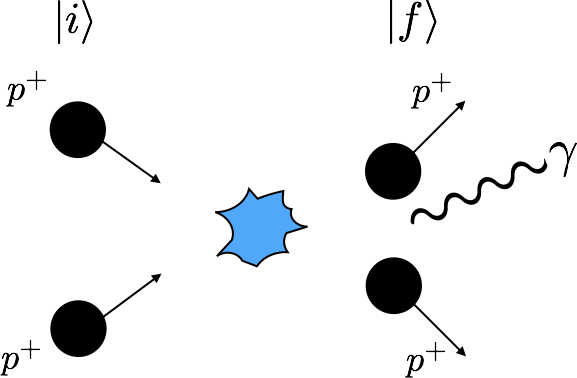
\includegraphics[width=.55\linewidth]{figures/QFT/istate_fstate.png}
\caption{An example of an initial state $\ket{i}$ with two incoming protons and a final state $\ket{f}$ with two outgoing protons and a photon $\gamma$. The blue object represents the interaction that takes place during the collision.}
\label{fig:ifstates}
\end{figure}
 The probability that the system evolves from state $\ket{i}$ into $\ket{f}$ is equal to the squared modulus of the amplitude,
\begin{equation}
\pif=|{\rm M}_{fi}|^{2},
\label{eq:Amp}
\end{equation}
and is in fact the only observation about a theory that can be made in physics experiments. After an initial and a final state are chosen, $\pif$ can be computed for a given QFT hypothesis and compared to the $\pif$ observed in experiment, and, depending on the consistency of the two answers, evidence can begin to build for or against the hypothesis. Commonly, $\pif$ is computed for two or more competing hypotheses, and the degree of consistency between each hypothesis and the experimental result are compared. In this way, a given hypothesis may be ``favored by the data'' relative to some other hypothesis, an idea that is further discussed in Chapter \ref{chap:run1pmssm}. Clearly, having a way to predict amplitudes is of utmost experimental importance. However, since most physicists are ultimately interested in understanding the physics that underlies the amplitude calculation\textemdash in other words, the physics that describes nature more deeply\textemdash a bit more detail is called for.


\section{Fields}

The primary degrees of freedom of a QFT are the fields. Mathematically, fields are single- or vector-valued functions of the spacetime coordinates, time and position in space. Physically, fields are interpreted as invisible objects that fill  space, taking on a density that varies from point to point, and sometimes an associated direction that likewise varies from point to point (Fig. \ref{fig:field}). A field can carry any number of properties, including energy, momentum, angular momentum, and charge density. When two or more fields interact, the relative local densities of the fields undergo changes, which can result in the the exertion of forces or the creation of matter.
\begin{figure}[h]
\centering
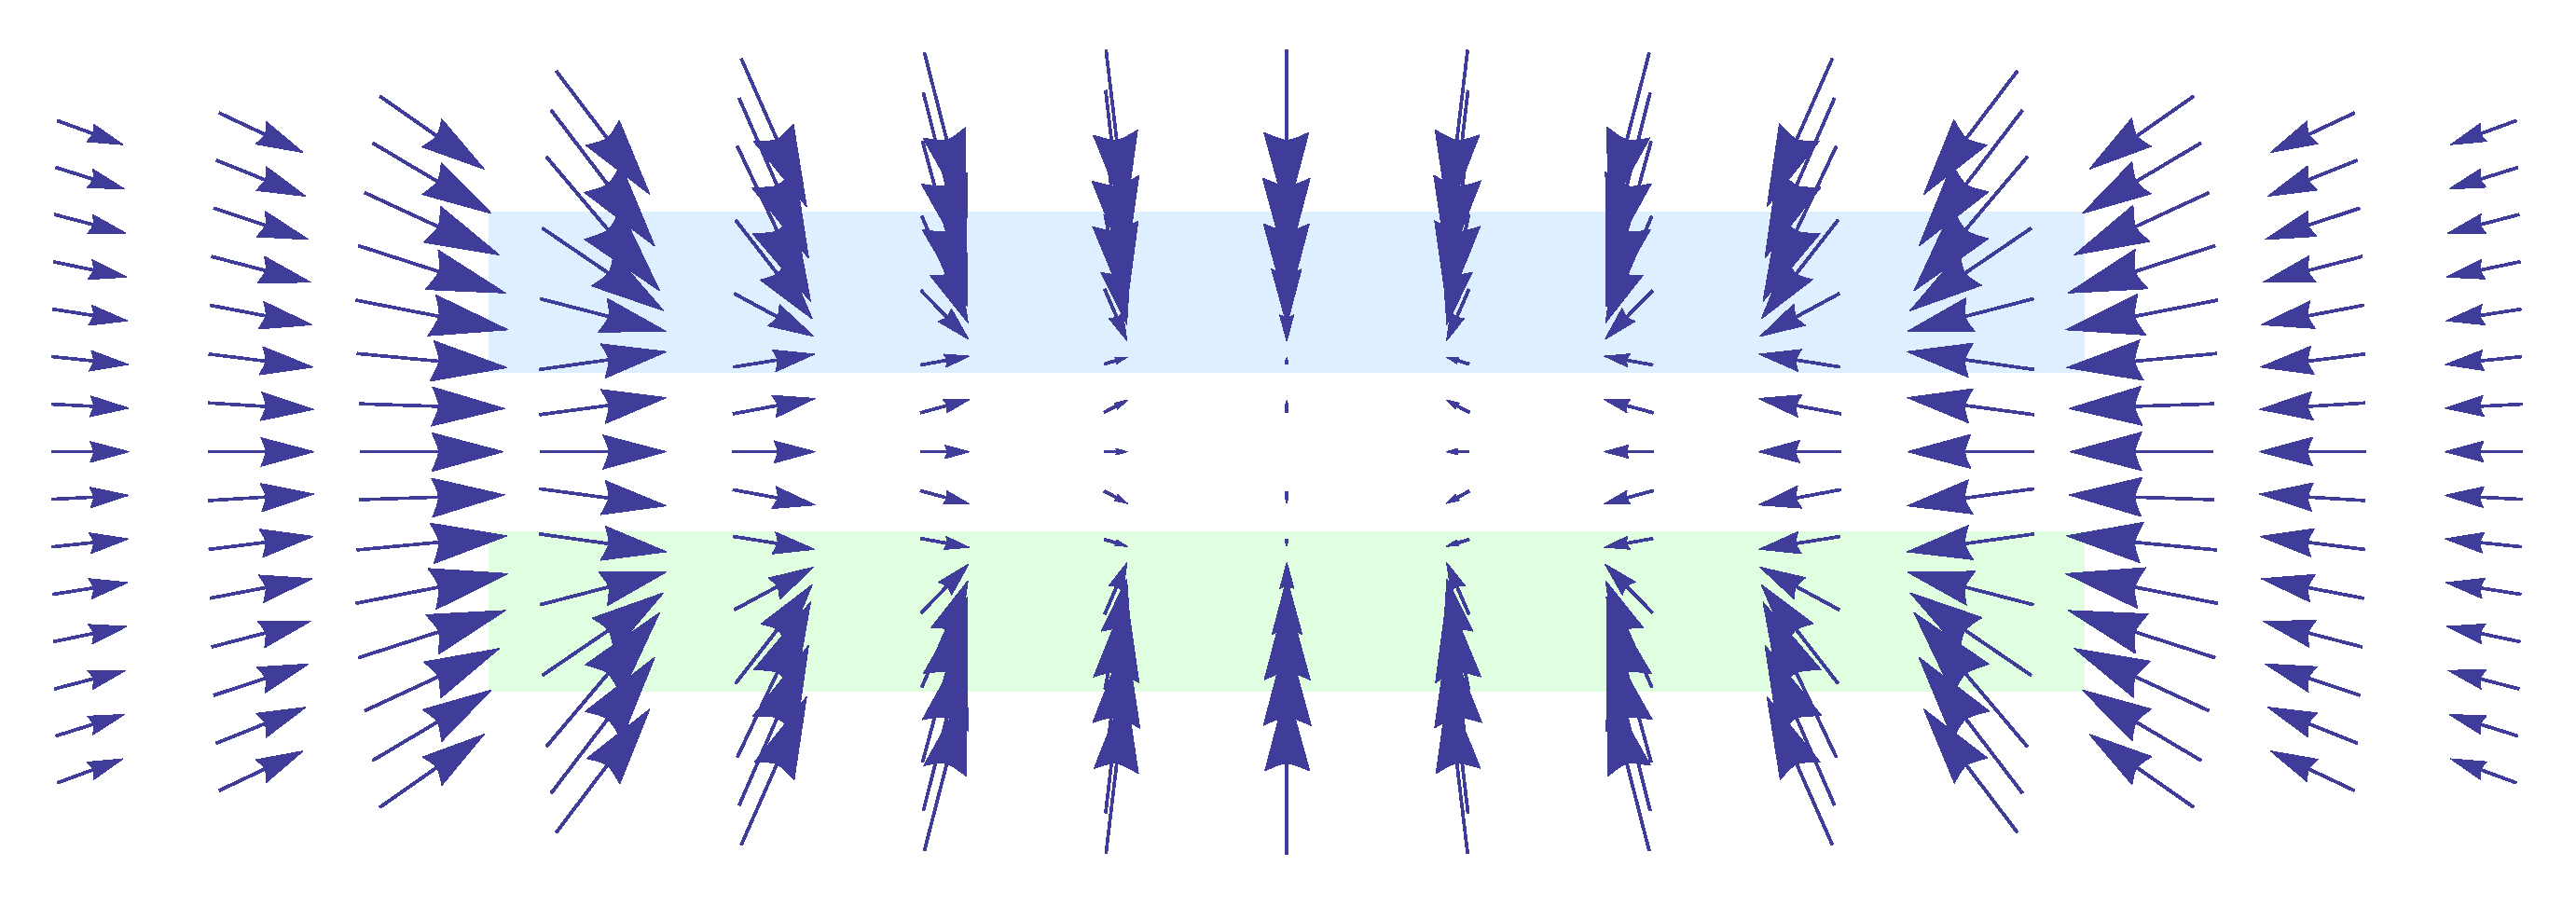
\includegraphics[width=.95\linewidth]{figures/QFT/GField.pdf}
\caption{An example of a field. The dark blue arrows show the magnitude and direction of the gravity field between two massive parallel plates shown in light blue and green. }
\label{fig:field}
\end{figure}

\section{Symmetry}
The way fields interact with one another depends on the set of symmetries that are present in the theory. Here, a symmetry is a property that ensures that some aspect of a system remains unchanged when the system is transformed in some way. Certain symmetries are inherent in every QFT, and these are the 10 non-spin related spacetime symmetries corresponding to the 10 generators of the Poincar{\'e} group~\cite{Peskin:1995ev}: 3 spatial translations and 1 time translation, 3 rotations,  and 3 boosts. Here, boosts are the generators of the Lorentz group, transforming a system from one inertial reference frame to another. All of these transformations correspond to invariant quantities, giving rise to the laws of the conservation of momentum, energy, angular momentum, and of the spacetime interval defined in special relativity. 

Other symmetries are referred to as internal or ``gauge" symmetries, and are free to be chosen during the construction of a QFT. An example of a gauge symmetry is the so-called unitary-1, or U(1), symmetry, which is respected by objects that do not change when they undergo planar rotations. In an abstract geometrical sense, circles respect U(1) symmetry because their shapes do not change when they are rotated about their centers by any angle; in the sense of a gauge symmetry, U(1) is notably respected by the QFT known as quantum electrodynamics (QED), the first successful QFT, because QED contains a parameter which, if rotated about the complex unit circle, yields back the same theory. 

The transformation of a field under a given symmetry can be represented by an operator $\hat{T}$, which is an object that changes (operates) on another object. The transformation on a field $\phi$ can be written as
\begin{equation}
\hat{T}[\phi] = \phi',
\end{equation}
where $\phi$ is the original field and $\phi'$ is the transformed field. The criterion for a theory to be invariant under a transformation $\hat{T}$ is that the Lagrangian density be unchanged after the replacement of the old fields by the transformed fields.

\section{Lagrangian density}
\label{sss:QFT}
 The mathematical object that encodes all the information in a perturbative (well-behaved) QFT is the Lagrangian density $\Lag$, sometimes just called the Lagrangian. The Lagrangian is a measure of the potential energy of a system subtracted from the kinetic energy, and is composed of terms proportional to the products of the field densities. The exact form of $\Lag$ follows from the set of fields and symmetries that are chosen in the QFT, and the various terms contain information about different physical processes. As an example, we examine the Lagrangian for a QFT in which there is only one field $\phi$, which is single valued (a scalar) and real. The Lagrangian density for this theory is given by
 \begin{equation}
 \Lag =  \frac{1}{2}(\partial_\mu \phi)^2  - a\phi^2 - b\phi^4,
 \label{eq:exLag}
 \end{equation} 
where a and b are constants and $\partial$ is the partial derivative taken with respect to the spatial coordinates. It is apparent that this Lagrangian is an expansion in powers of the field, and this is a general feature of Lagrangians; they are in fact Taylor expansions in the fields. 

The concept of symmetry can be illuminated in the context of this Lagrangian, because $\Lag$ can be seen to respect a particular symmetry called $\ztwo$ symmetry. $\ztwo$ symmetry is the invariance of a system under the operation of reversing the sign of the fields. In other words, a Lagrangian that respects a $\ztwo$ symmetry is invariant under the operation of $\hat{T}$, where $\hat{T}$ is defined by 
\begin{equation}
\hat{T}[\phi] \equiv \phi' = -\phi.
\end{equation}
All terms in this Lagrangian contain even powers of the field $\phi$, and so all minus signs brought about by the operation of $\hat{T}$ on $\Lag$ cancel, giving back the original Lagrangian:
 \begin{align}
 \begin{split}
\hat{T}[\Lag] \equiv \Lag' &= -\frac{1}{2}\partial_\mu (-\phi) \partial^\mu (-\phi)  - a(-\phi)^2 - b(\phi)^4 \\
&= -\frac{1}{2}\partial_\mu \phi \partial^\mu \phi  - a\phi^2 - b\phi^4 \\
&= \Lag.
 \label{eq:exLag2}
  \end{split}
\end{align} 
If $\Lag$ had contained a term proportional to $\phi^3$, the theory would not respect a $\ztwo$ symmetry, because $\hat{T}[\Lag]$ would not yield back $\Lag$.

As stated, each term in the Lagrangian carries specific physical meaning. The first term in Equation \ref{eq:exLag} accounts for the kinetic energy stored in the field, the second term accounts for particle mass, and the third term is an interaction term. These points are discussed now.

\section{Particles (quadratic term)}
A field typically exhibits a resonance at an energy value proportional to the coefficient of the quadratic term in the Lagrangian; in this case, twice the value of a. This resonance is referred to as a particle, and has a mass defined by the energy of the resonance:
\begin{equation}
m_{\phi} = 2a.
\end{equation}
Particles are localized quanta, or pieces, of the fields, and they carry the same properties as the fields. These properties include energy $E$ and momentum components $p_i$ ($i=x,y,z$), which can be combined into a single object called a four-vector,
\begin{equation} 
p^\mu=(E,p_x,p_y,p_z)^\mu,
\end{equation}
whose magnitude is invariant under Lorentz transformations; particles can also carry charge, a property that is invariant under gauge transformations; and they have spin, where spin is the ``intrinsic'' angular momentum possessed by a particle in the absence any interaction taking place. The smallest natural increment of spin is equal to half of Planck's constant $\hbar$, and thus all particles have a spin equal to an integer multiplied by this unit:
\begin{equation}
s_\phi = N\cdot \frac{\hbar}{2}.
\end{equation}
Particles for which $N$ is an even integer are called bosons, and those with an odd $N$ are called fermions. The bosonic or fermionic nature of particles in a system determines many bulk properties of the system, most importantly whether or not the particles can be arranged to form rigid structures; fermions are able to do so, and bosons are not.
%Whether a particle is a boson or a fermion determines many properties about that particle, including notably whether it can occupy %don't think I need this

\section{Feynman diagrams (interaction terms)}
\label{sec:withztwo}
As mentioned in Section \ref{sec:Amp}, the primary role of QFT from an experimental point of view is to predict amplitudes. To a first approximation, the amplitude for a system to evolve from state $\ket{i}$ to state $\ket{f}$ is given by the quantity
\begin{equation}
{\rm M}_{fi}=\bra{f}\hat{H}\ket{i},
\end{equation}
where the time evolution operator $\hat{H}$ can be derived from the Lagrangian. 
%In this expression, $\hat{H}$ acts on and modifies the state $\ket{i}$, the resulting state is projected onto the final state $\ket{f}$, and this yields the amplitude. % maybe won't need
There are various methods for computing this amplitude, but the most widely used is Feynman's method. Feynman's method amounts to doing a perturbative expansion over the possible ways (modes) for the state $\ket{i}$ to transform into state $\ket{f}$. Each possible mode is weighted by a number that can be computed from a diagram, and after the partial amplitudes for all possible diagrams have been computed, they are added together to form the amplitude M$_{fi}$. By Equation \ref{eq:Amp} the square of the amplitude yields the probability for state $\ket{i}$ to evolve into state $\ket{f}$.

\begin{figure}[h]
\centering
%\hspace{0cm}f
\subfloat[allowed]{
  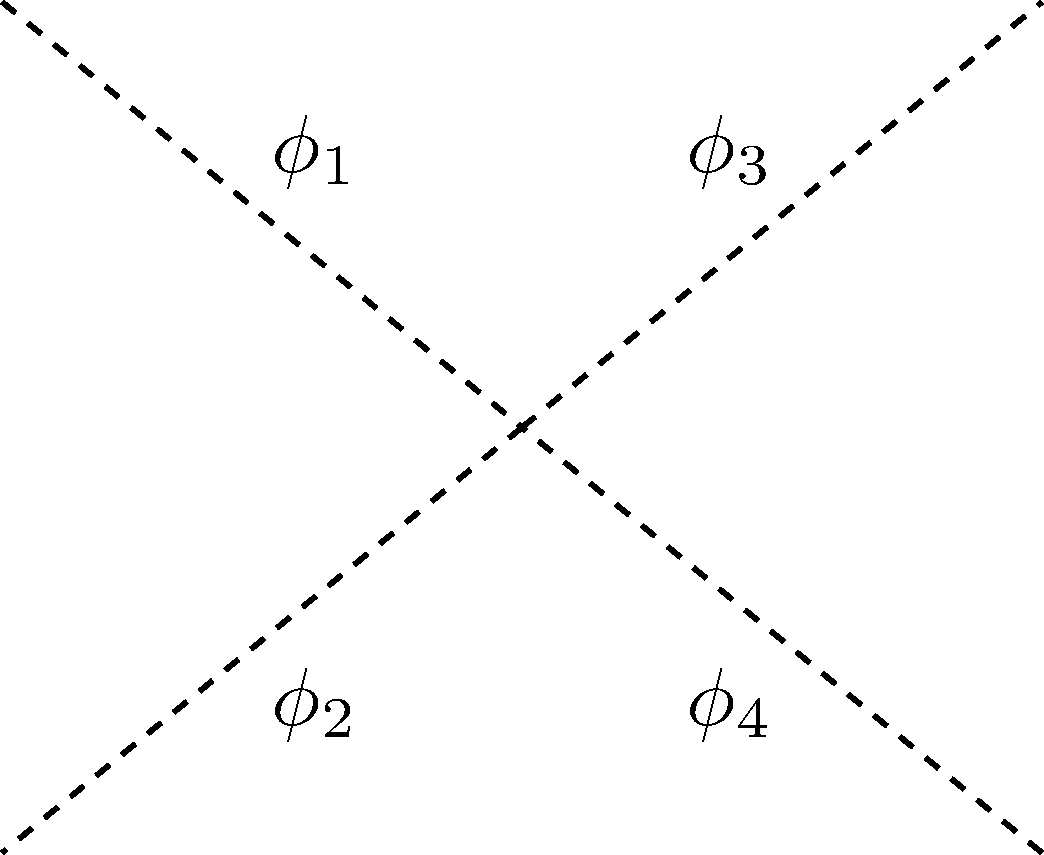
\includegraphics[width=0.32\linewidth]{figures/QFT/feyn1}
}
%\hspace{1cm}
\subfloat[allowed]{
  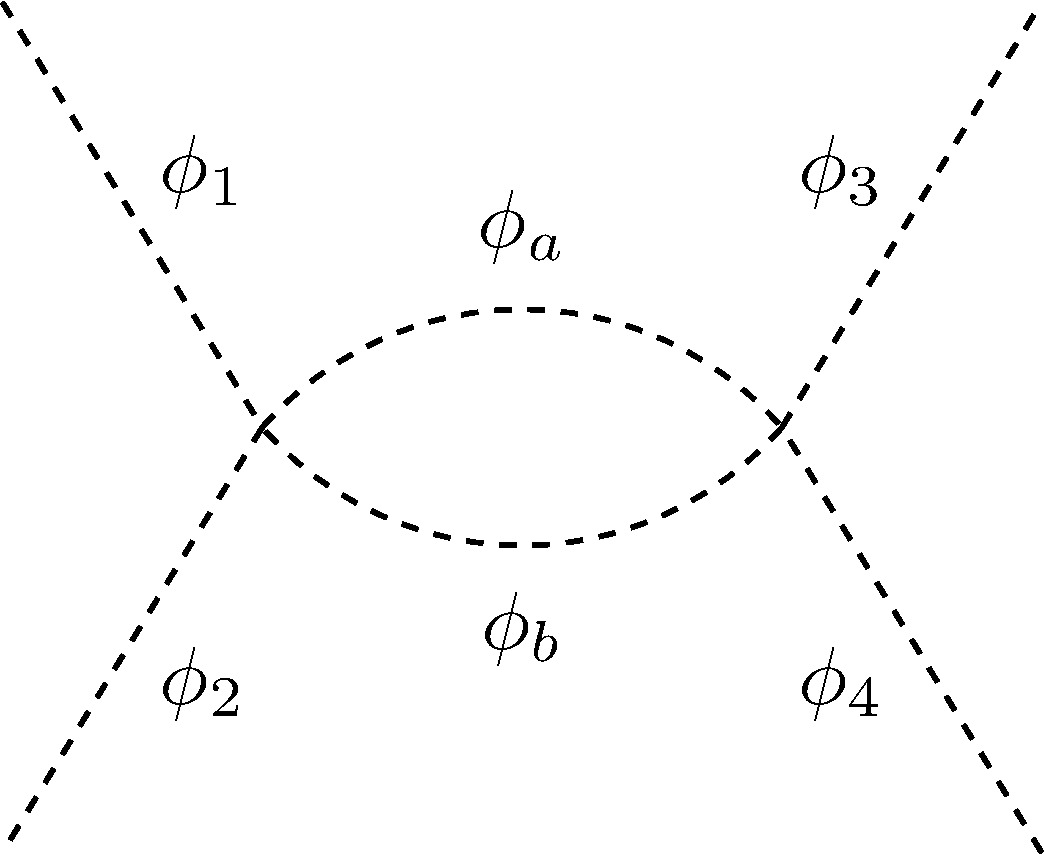
\includegraphics[width=0.32\linewidth]{figures/QFT/feyn2}
}
%\\
\subfloat[forbidden before SSB]{
  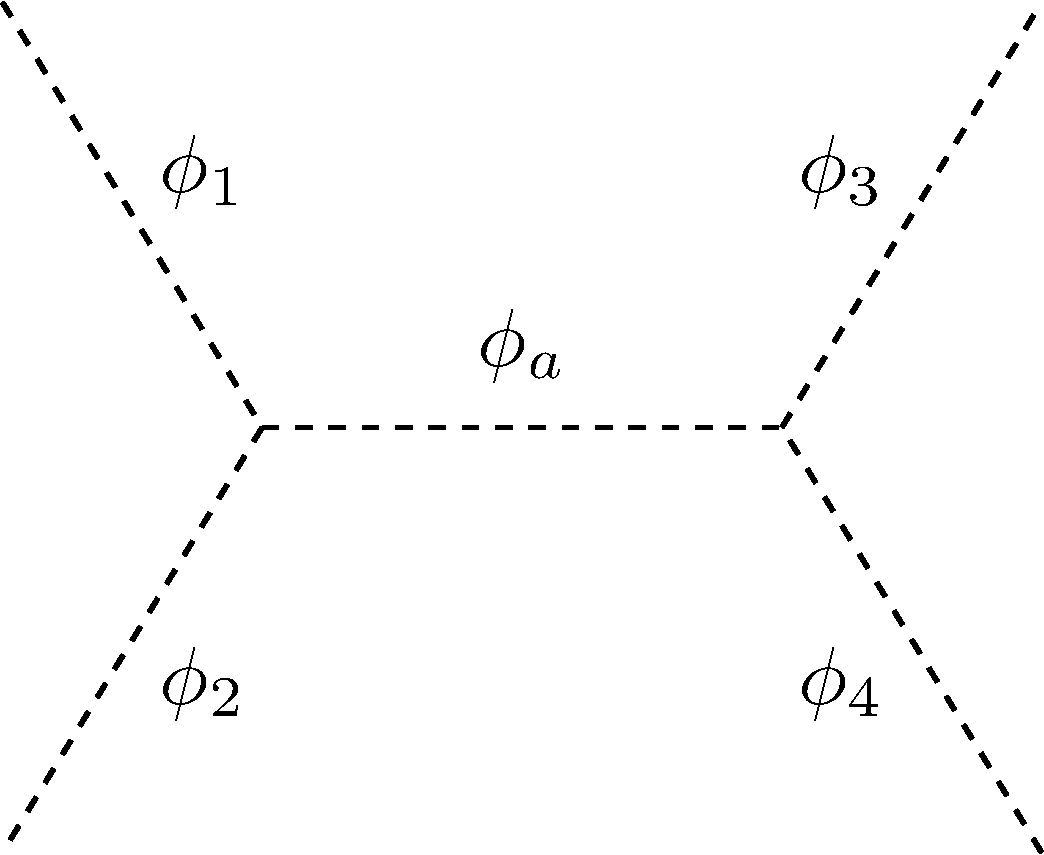
\includegraphics[width=0.32\linewidth]{figures/QFT/feyn3}
}
\caption{Diagrams a and b are two of the leading Feynman diagrams in the theory defined by Equation \ref{eq:exLag}. Diagram c is forbidden by the theory, and so does not contribute to the amplitude. }
\label{fig:Feyn}
\end{figure}

Suppose, for example, we are working within the theory defined by the Lagrangian in Equation \ref{eq:exLag}, that the initial state $\ket{i}$ consists of two identical incoming particles $\phi_1$ and $\phi_2$, and that the final state $\ket{f}$ consists of two outgoing particles $\phi_3$ and $\phi_4$. Figure \ref{fig:Feyn} 
shows two of the leading Feynman diagrams (a and b), each representing a possible mode for the specified process, and one diagram c that is not allowed by the theory. Each allowed diagram contributes a partial amplitude, and the sum of all partial amplitudes is the total amplitude M$_{fi}$. The two essential features of these and any Feynman diagrams are:
\begin{itemize}
\item lines, which represent particles of the field $\phi$, where dashes signify that in this case the particles have no spin, and
\item vertices, which are the fundamental interactions between particles.  
\end{itemize}
By convention, time flows horizontally, and so the initial state consists of the particles on the left side of a diagram, and the final state consists of the particles on the right side. Diagrams a and c are called tree level diagrams because they appear to have branches that do not close to form loops. Diagram b, by contrast, contains an internal loop of particles, and so is not a tree-level diagram. Tree-level diagrams typically yield the largest partial amplitudes, and thus are often the most important.

The guiding principle for constructing diagrams is that any diagram not forbidden by the theory will, in principal, contribute to the total amplitude. Allowed diagrams are those for which every vertex within a diagram is associated with a term in the Lagrangian. For our $\Lag$, the only interaction term is the quartic term, $c\phi^4$, and this term gives rise to the four-particle vertex seen in the center of the diagram in Fig. \ref{fig:Feyn} (a). This can be generalized, since a term in a Lagrangian proportional to n powers of a field gives rise to an n-particle vertex in the theory. The more complicated diagram in Fig. \ref{fig:Feyn} (b) is built out of two copies of the four-particle vertex, and so is allowed. One could imagine a vertex of only three $\phi$ particles, shown in Fig. \ref{fig:Feyn} c. However, the three-particle vertex does not correspond to any term in the Lagrangian. For such a vertex to exist, $\Lag$ would have to contain a term proportional to $\phi^3$, and it was already established that such a term would violate the $\ztwo$ symmetry respected by the theory. Therefore, the three-particle vertex, and diagram c, are forbidden by symmetry, and so do not enter into the amplitude calculation. 

In principle, one should construct and compute all possible diagrams and amplitudes, of which there are an infinite number, but this turns out to be unnecessary if the goal is to make reasonably accurate predictions. The simplest diagrams\textemdash the tree-level diagrams\textemdash typically give the largest contribution to the amplitude because they have fewer vertices than do more complicated diagrams. Each vertex contributes a factor of $4!\cdot b$ to the partial amplitude, and provided that $4!\cdot b$ is always less than 1,  diagrams with more vertices yield smaller partial amplitudes. Taking an approximation where only the tree-level diagrams (diagram a) contribute, the amplitude and probability are given by\footnote{For a complete description of the Feynman rules, see \cite{Peskin:1995ev}.}:
\begin{align}
%\begin{split}
&{\rm M}_{fi}=-(4!)\ b,\\
&\pif = (-4!)^2\ b^2 = 576\ b^2.
%\end{split}
\end{align}
The quantity $(4!)b$ is sometimes referred to as a coupling constant, $\lambda$, named so because its value dictates the strength of the amplitude associated with the interaction. A couple of observations: first, the amplitude contains a single power of the constant b, because the contributing diagram has only a single vertex. Second, a notable feature of the probability is that $\pif$ is constant with respect to all kinematic properties of the outgoing particles. This means that if many collisions were to occur in succession, the distribution of the final state particles would be isotropic. Of course, this is a conclusion reached by analyzing the leading order contributions. If diagram b or other higher-order diagrams had been included, the prediction of isotropic final states might not have been absolute, but any deviation from this behavior would be suppressed by additional factors of b. 

\section{Conserved quantities}
Noether's theorem \cite{Noether:1918zz} states that every continuous symmetry respected by a theory is associated with some conserved quantity, and the same is often true in the case of discrete symmetries. It was established that the QFT at hand respects a $\ztwo$ symmetry, so what is the associated conserved quantity? The answer can be deduced through a bit of analysis of the interaction terms of the Lagrangian. In $\Lag$, terms with an even number of powers of the field are present, which means that vertices involving an even number of particles are allowed. However, terms with odd powers of the fields are not present, which means that vertices with an odd number of particles are not allowed. This fact means that while it is possible for a pair of particles to be created or destroyed, the same is not true for a single particle. If the initial number of particles is even, the final number will also be even; if the initial number is odd, the final number will be odd. The conserved quantity is:
\begin{equation}
\theta = n\pmod{2},
\label{eq:theta}
\end{equation}
where $n$ is the number of particles in the system. In this theory, the value of $\theta$ for an isolated system can never change.

\section{Symmetry breaking}
The previous analysis of the scalar Lagrangian was valid but not unique. It was assumed that the parameters $a$ and $b$ were positive, but it happens that the dynamics of the theory change considerably if the parameter $a$ takes on a negative value. Since the Lagrangian is constructed as the difference between the kinetic and potential energy of the system, the second and third term define a potential energy V:
\begin{equation}
V(\phi) = a\phi^2 + b\phi^4.
\end{equation}
For positive $a$, $V(\phi)$ exhibits a minimum at the value $\phi=0$, as seen in Fig. \ref{fig:SSB} (a) and (b). But if $a$ is negative, $V(\phi)$ exhibits two minima, located at 
\begin{equation}
\phi_{min} \equiv {\rm VEV} = \pm \sqrt{\frac{a}{2b}},
\end{equation}
where VEV is the vacuum expectation value, that is, the average value of the field in the vacuum.
\begin{figure}[h]
\centering
\hspace{-0.3cm}
\subfloat[$a>0$]{
  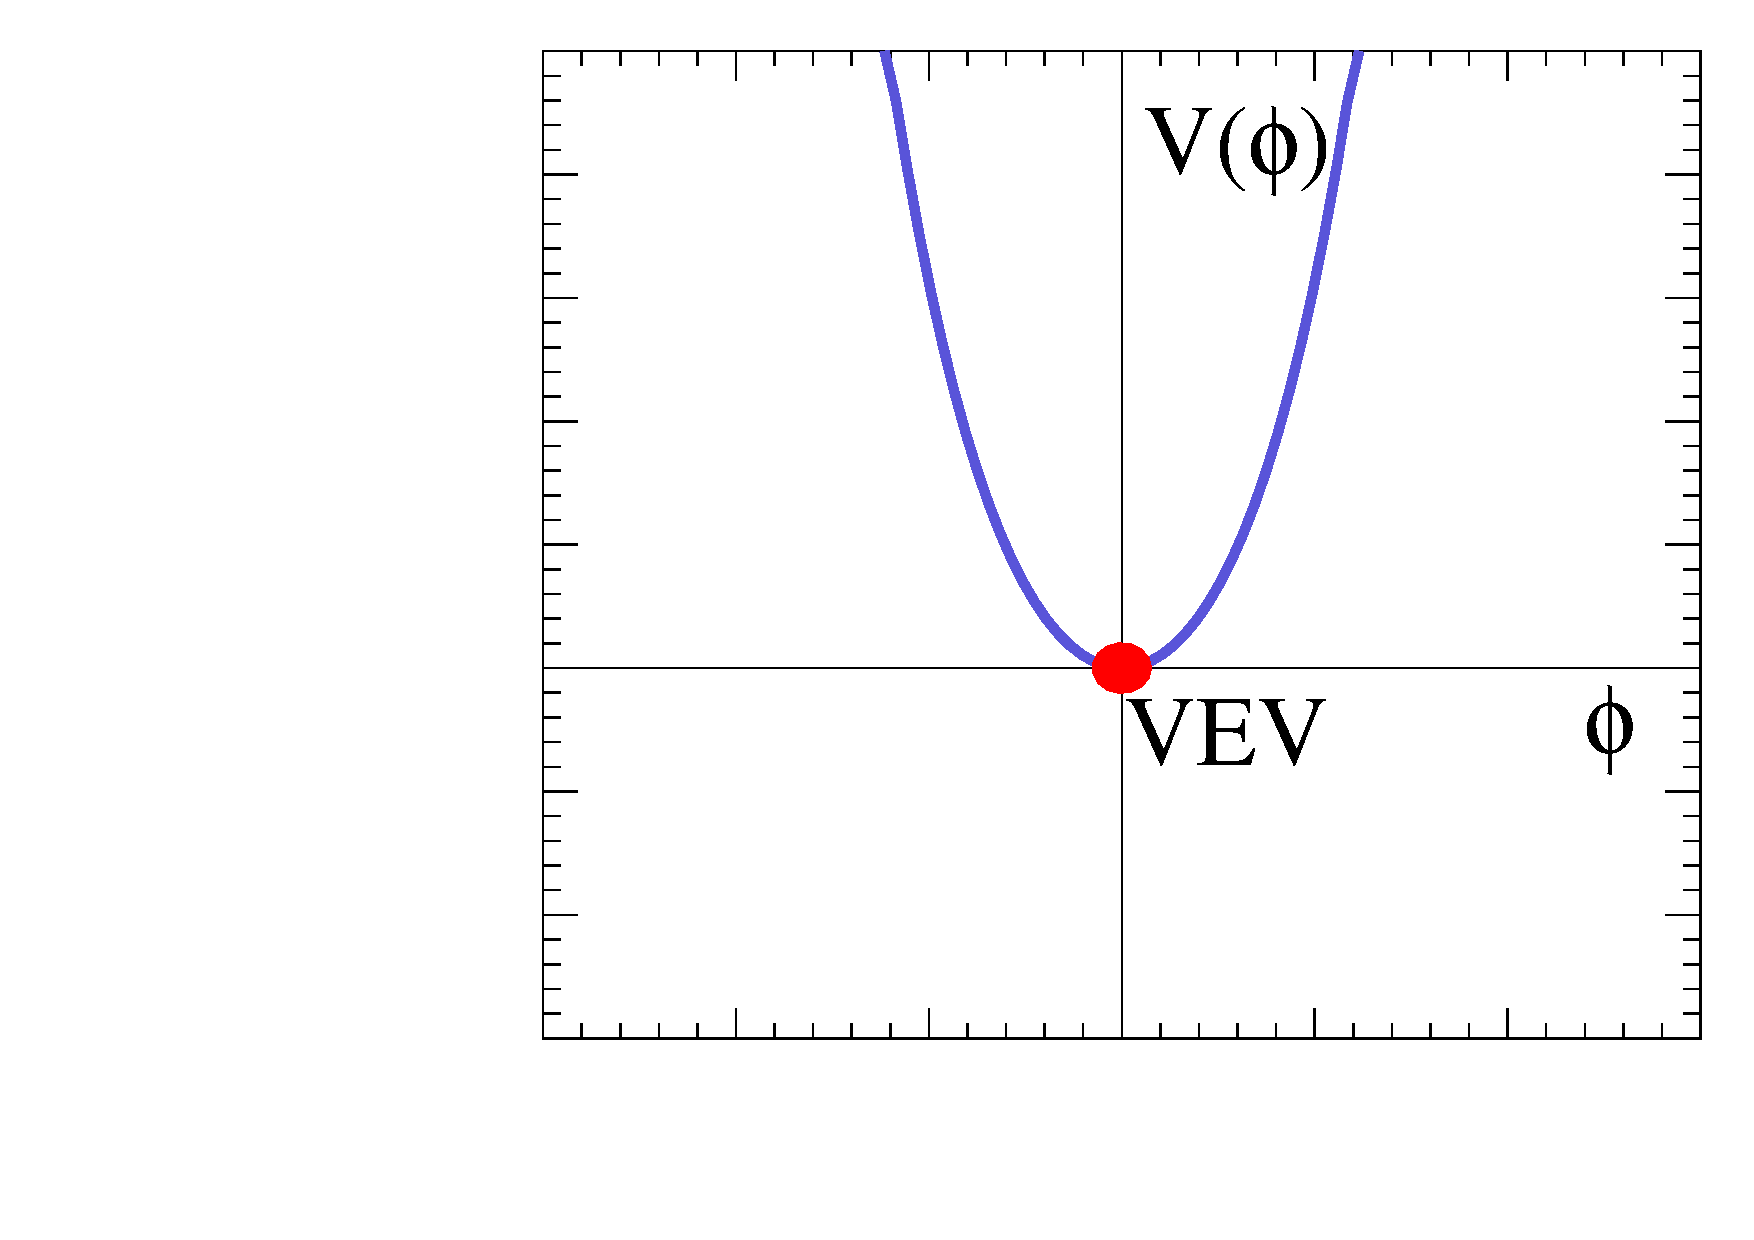
\includegraphics[width=0.33\linewidth]{figures/QFT/SB1.pdf}
}
\hspace{-0.3cm}
\subfloat[$a=0$]{
  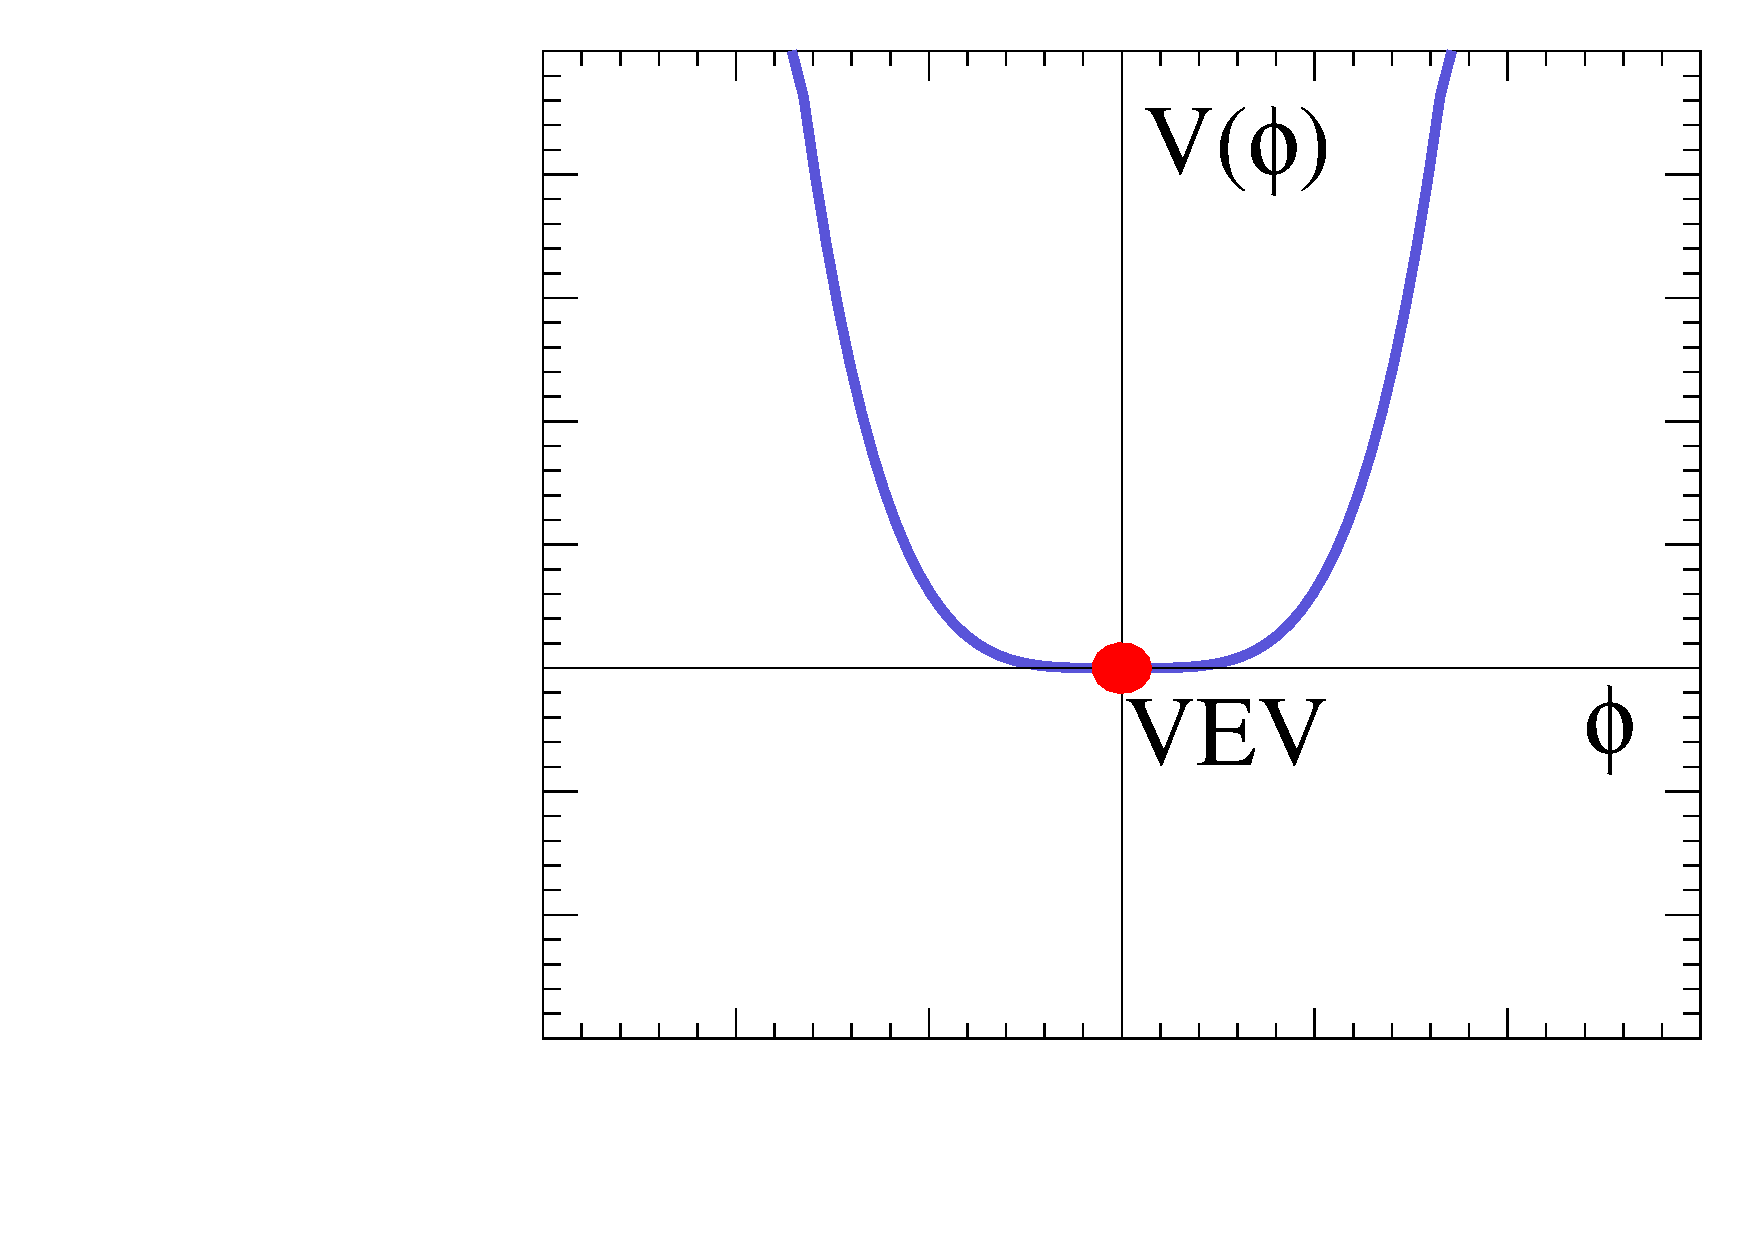
\includegraphics[width=0.33\linewidth]{figures/QFT/SB2.pdf}
}
\hspace{-0.3cm}
\subfloat[$a<0$]{
  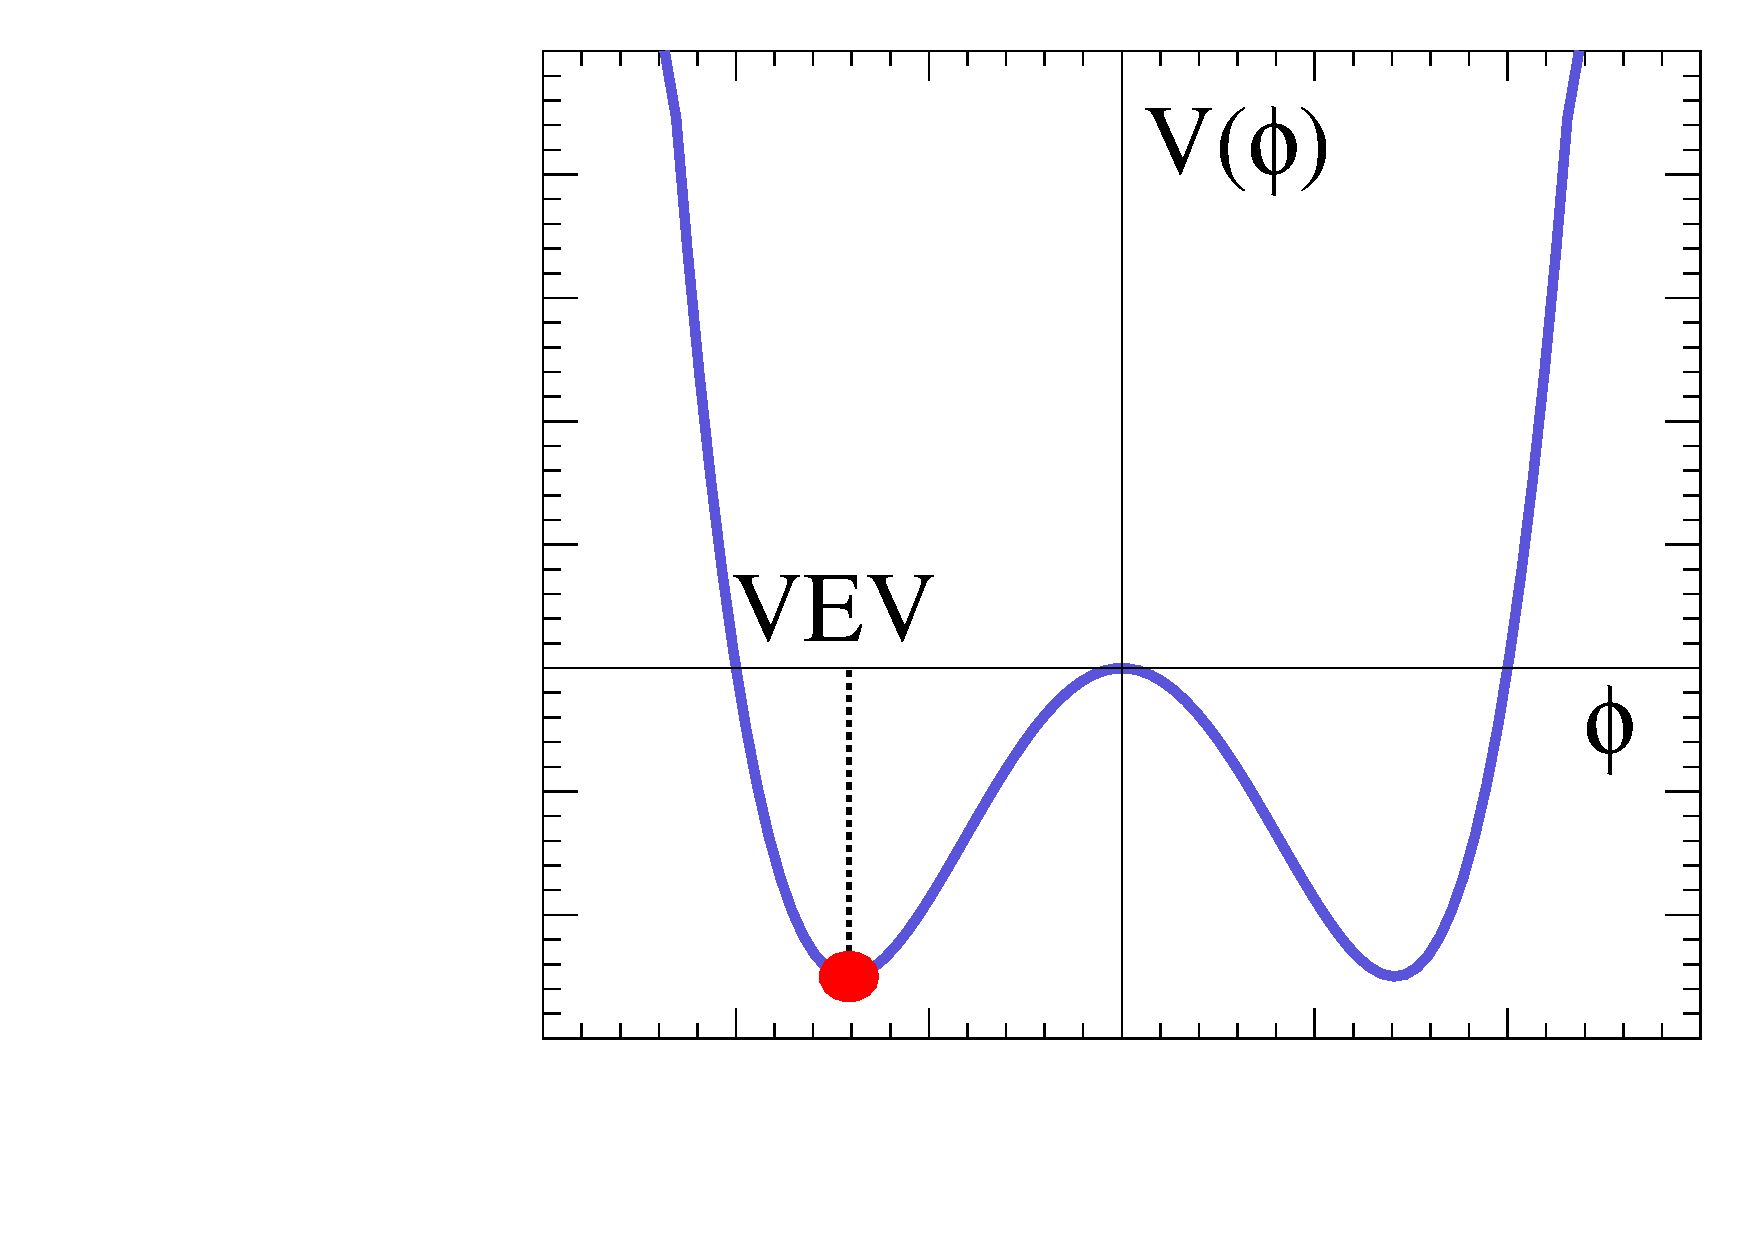
\includegraphics[width=0.33\linewidth]{figures/QFT/SB3.pdf}
}
\caption{The shape of the potential for three choices of parameter a: positive, zero, and negative. The field $\phi$ always centers on a local minimum of the potential, which is marked in the three cases by the red dot. }
\label{fig:SSB}
\end{figure}

Physical systems tend to evolve towards a state of lower energy, and so it is no surprise that the appearance of these energy minima leads to a qualitative change in the behavior of the system.  The field density will naturally settle into one of these minima, located at an energy value equal to the VEV. When this happens, a visible change takes place at the level of the Lagrangian. The field $\phi$ splits into a static component equal to the VEV, and a dynamic part, which is the modified field $\phitwo$:
\begin{equation}
\phi \rightarrow {\rm VEV}+\phitwo.
\end{equation}
The Lagrangian in Equation \ref{eq:exLag} becomes
\begin{align}
\begin{split}
\Lag \rightarrow& -\frac{1}{2}(\partial_\mu [{\rm VEV}+\phitwo])^2  - a[{\rm VEV}+\phitwo]^2 - b[{\rm VEV}+\phitwo]^4\\
 = &\ \frac{1}{2}(\partial_\mu \phitwo)^2 - (a {\rm VEV}^2 + b {\rm VEV}^4) - (2 a {\rm VEV} + 4 b {\rm VEV}^3) \phitwo \\
& \ \ \ \ \ \ \ \ \ \ \ \ \ \ \ \ \  - (a + 6 b {\rm VEV}^2) \phitwo^2 - 4 b {\rm VEV} \phitwo^3 - b \phitwo^4 
\equiv \Lag_{\rm broken}.
 \end{split}
\end{align}
The terms without any powers of $\phitwo$ are non-physical and so can be ignored, and through a renaming of the constants, the Lagrangian can be written as
\begin{equation}
\Lag_{\rm broken} = \frac{1}{2}(\partial_\mu \phitwo)^2 - \alpha \phitwo^2 - \gamma \phitwo^3 - \beta \phitwo^4.
\end{equation}
Note that $\Lag_{\rm broken}$ closely resembles the original Lagrangian $\Lag$, but differs in a few key ways. For one, the coefficients of the quadratic and quartic terms have changed from $a$ and $b$ to $\alpha$ and $\beta$, where the latter depend on the magnitude of the symmetry breaking (the VEV). This means that the mass and coupling strength of the four-particle vertex have changed, which will ultimately result in a re-scaling of $\pif$. 

Then, the fact that there is now a cubic term ($\gamma \phitwo^3$) is particularly significant. In $\Lag$, the cubic term was explicitly forbidden by the $\ztwo$ symmetry, but upon the introduction of a non-zero VEV, $\ztwo$ is no longer respected. The symmetry is said to have been ``spontaneously broken.''  As a result of the emergent cubic term, the theory has a new allowed vertex of three particles, and so the interaction in the diagram of Fig. \ref{fig:Feyn} c is no longer forbidden! This changes the prediction for the amplitude, which now has four contributing tree-level diagrams instead of just one. The probability now depends on the the kinematics of the particles, and so the outgoing particles will no longer be distributed isotropically. Clearly, symmetry breaking has changed the physics considerably.

Perhaps the most striking change brought about by the breaking of the $\ztwo$ symmetry is that the previously conserved quantity $\theta$ (in Equation \ref{eq:theta}) is no longer conserved. Through processes involving the new three-particle vertex, the system can now start out with an even number of particles and end up with an odd number, or vice versa. Indeed, symmetry breaking is seen to have fundamentally changed the physics.

The concept of spontaneous symmetry breaking (SSB) is particularly relevant for the $\SM$ because it is key to the mechanism by which all the particles in the $\SM$ acquire mass, known as the Brout-Englert-Higgs mechanism \cite{Higgs:1964pj}. Before proceeding to describe the $\SM$, there is one last concept that must be mentioned, and that is of commutation relations.

\section{Commutation relations}
Symmetries are defined by an invariance under the action of an operator, and operators are defined by a set of commutation relations. In other words, they are defined by how they transform the states they act on, and by how they behave when applied in sequence with other operators. In general, the commutator and anticommutator of two operators $\hat{T}_1$ and $\hat{T}_2$ are defined by
\begin{align}
[\hat{T}_1,\hat{T}_2]\phi &\equiv \hat{T}_1 (\hat{T}_2 \phi)  - \hat{T}_2 (\hat{T}_1 \phi) \text{\ and}\\
\{\hat{T}_1,\hat{T}_2\}\phi &\equiv \hat{T}_1 (\hat{T}_2 \phi)  + \hat{T}_2 (\hat{T}_1 \phi),
\end{align}
respectively. Broadly speaking, boson fields commute, meaning their commutators are equal to 0, and fermion fields anticommute, meaning their anticommutators are equal to 0. For more information on commutators and QFT, please see Ref.~\cite{Peskin:1995ev}.

The reader has now received an entertaining yet strategic introduction to the basic concepts and vocabulary that will be necessary to describe the $\sm$ and what seems to be the endless search for supersymmetry.



